\chapter{Конструкторская часть}

\section{Используемые типы и структуры данных}

Для работы программы потребуются следующие структуры данных:

\begin{itemize}
	\item четырёхмерный вектор, состоящий из 4 чисел с плавающей точкой. Требуется для преобразования координат точки для последующей отрисовки. Четвёртая координата нужна для получения перспективной проекции;
	\item трехмерный вектор, состоящий из 3 чисел с плавающей точкой. Требуется для вычисления нормалей, а также для хранения точек;
	\item матрица размером 4 на 4, состоящая из 16 чисел с плавающей точкой. Требуется для перевода точек в нужный базис;
	\item камера. Состоит из позиции (трехмерный вектор), базиса (3 трехмерных вектора), фокусного расстояния (число с плавающей точкой) и дальности прорисовки (число с плавающей точкой);
	\item источник света, состоящий из 2 углов (2 числа с плавающей точкой);
	\item ландшафт. Состоит из карты высот (двумерный словарь точек, ключами являются числа с плавающей точкой) и похожей карты квадратов. Каждый из квадратов, в свою очередь, является двумерным квадратным массивом точек;
	\item сцена, содержащая в себе все остальные объекты.
\end{itemize}

\section{Структура программы}

Функциональная схема работы программы приведена в приложении А.

Также для снижения сложности модификации было принято решение использовать парадигму объектно-ориентированного программирования и паттерны проектирования. Диаграмма классов представлена на рисунке \ref{fig:classes}

\begin{figure}[h!]
	\centering
	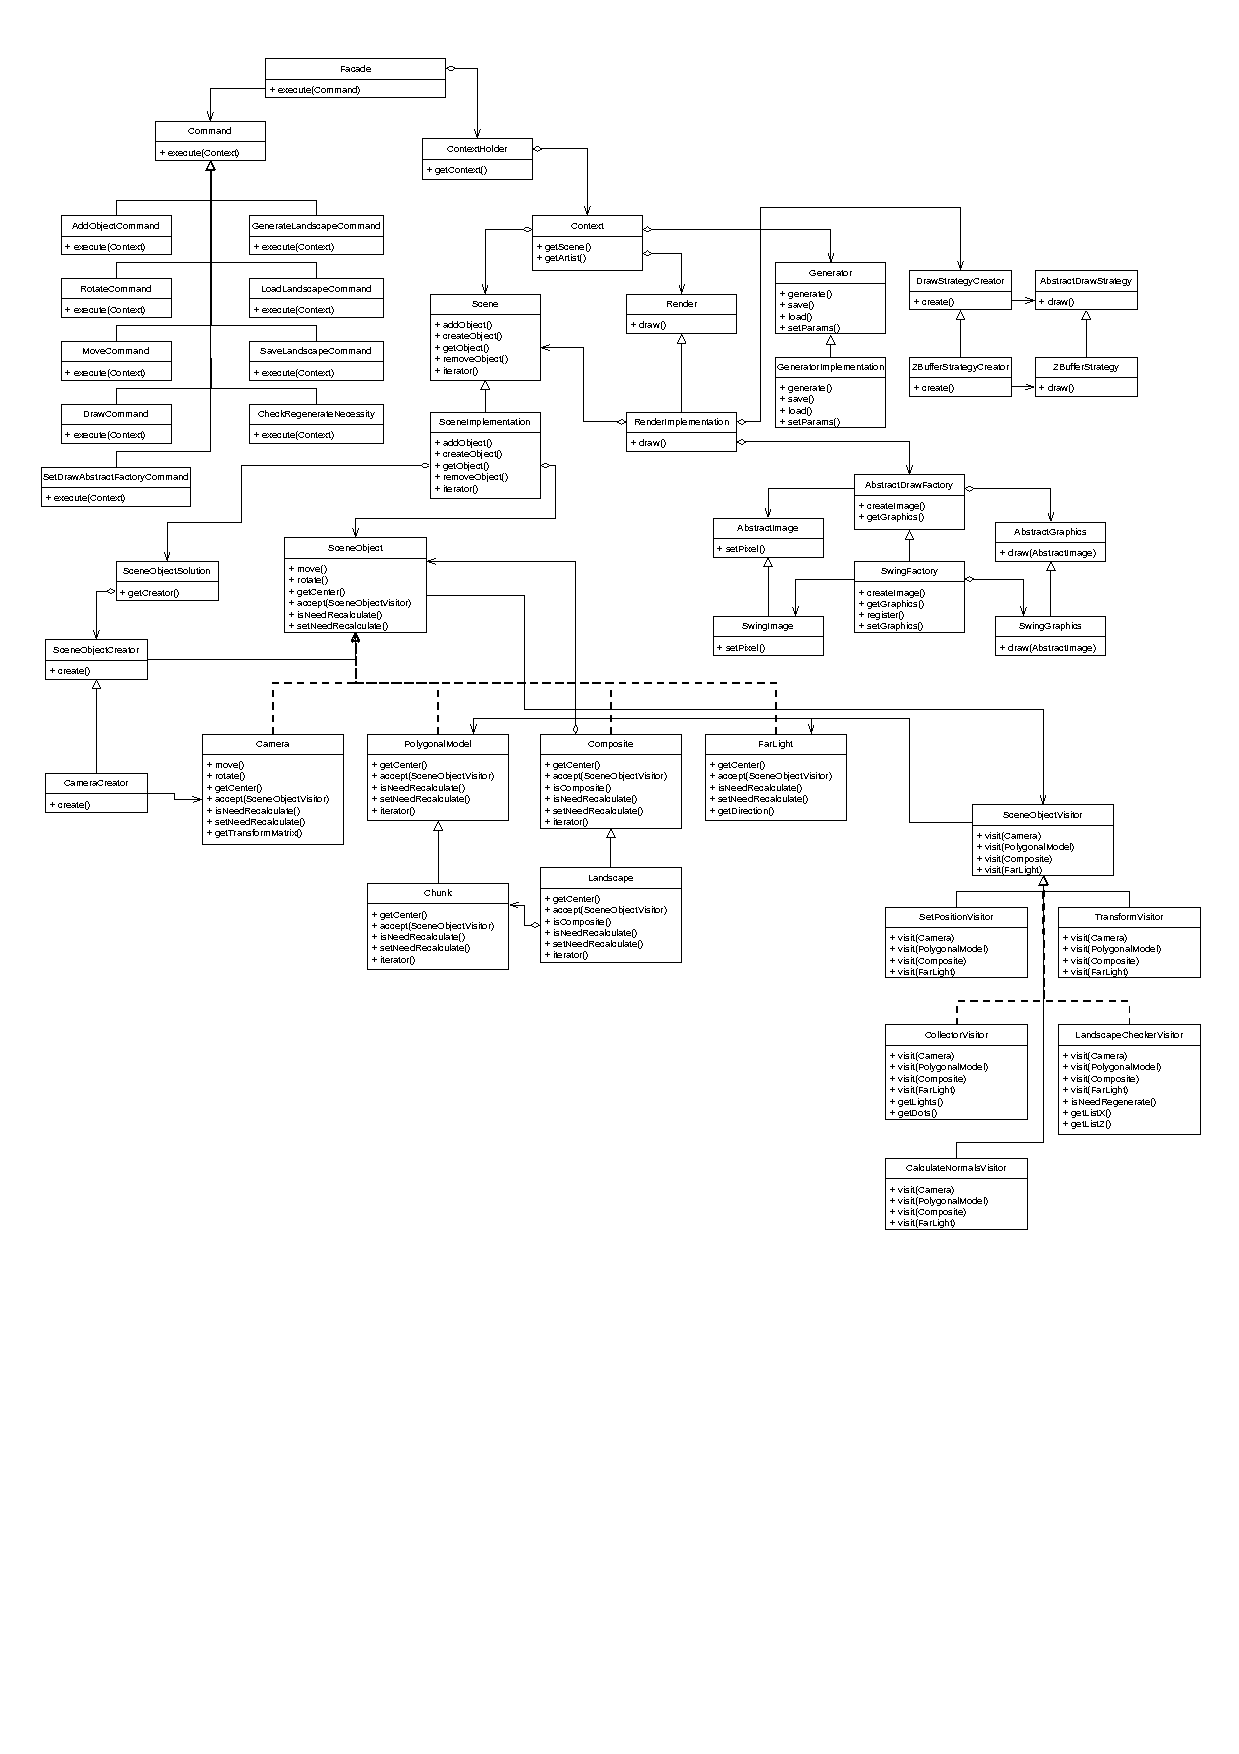
\includegraphics[width=0.9\textwidth]{tex_parts/diagram.pdf}
	\caption{\label{fig:classes}Диаграмма классов}
\end{figure}


\section{Схемы алгоритмов генерации ландшафта}

На вход каждому алгоритму подаётся диапазон высот, дальность и шаг отрисовки, а также положение камеры. Сторону квадрата примем за 1024 из-за ограничений алгоритма diamond-square. 

\subsection{Алгоритм diamond-square}

Схема алгоритма представлена на рисунке \ref{fig:ds-scheme}. 

\begin{figure}[h!]
	\centering
	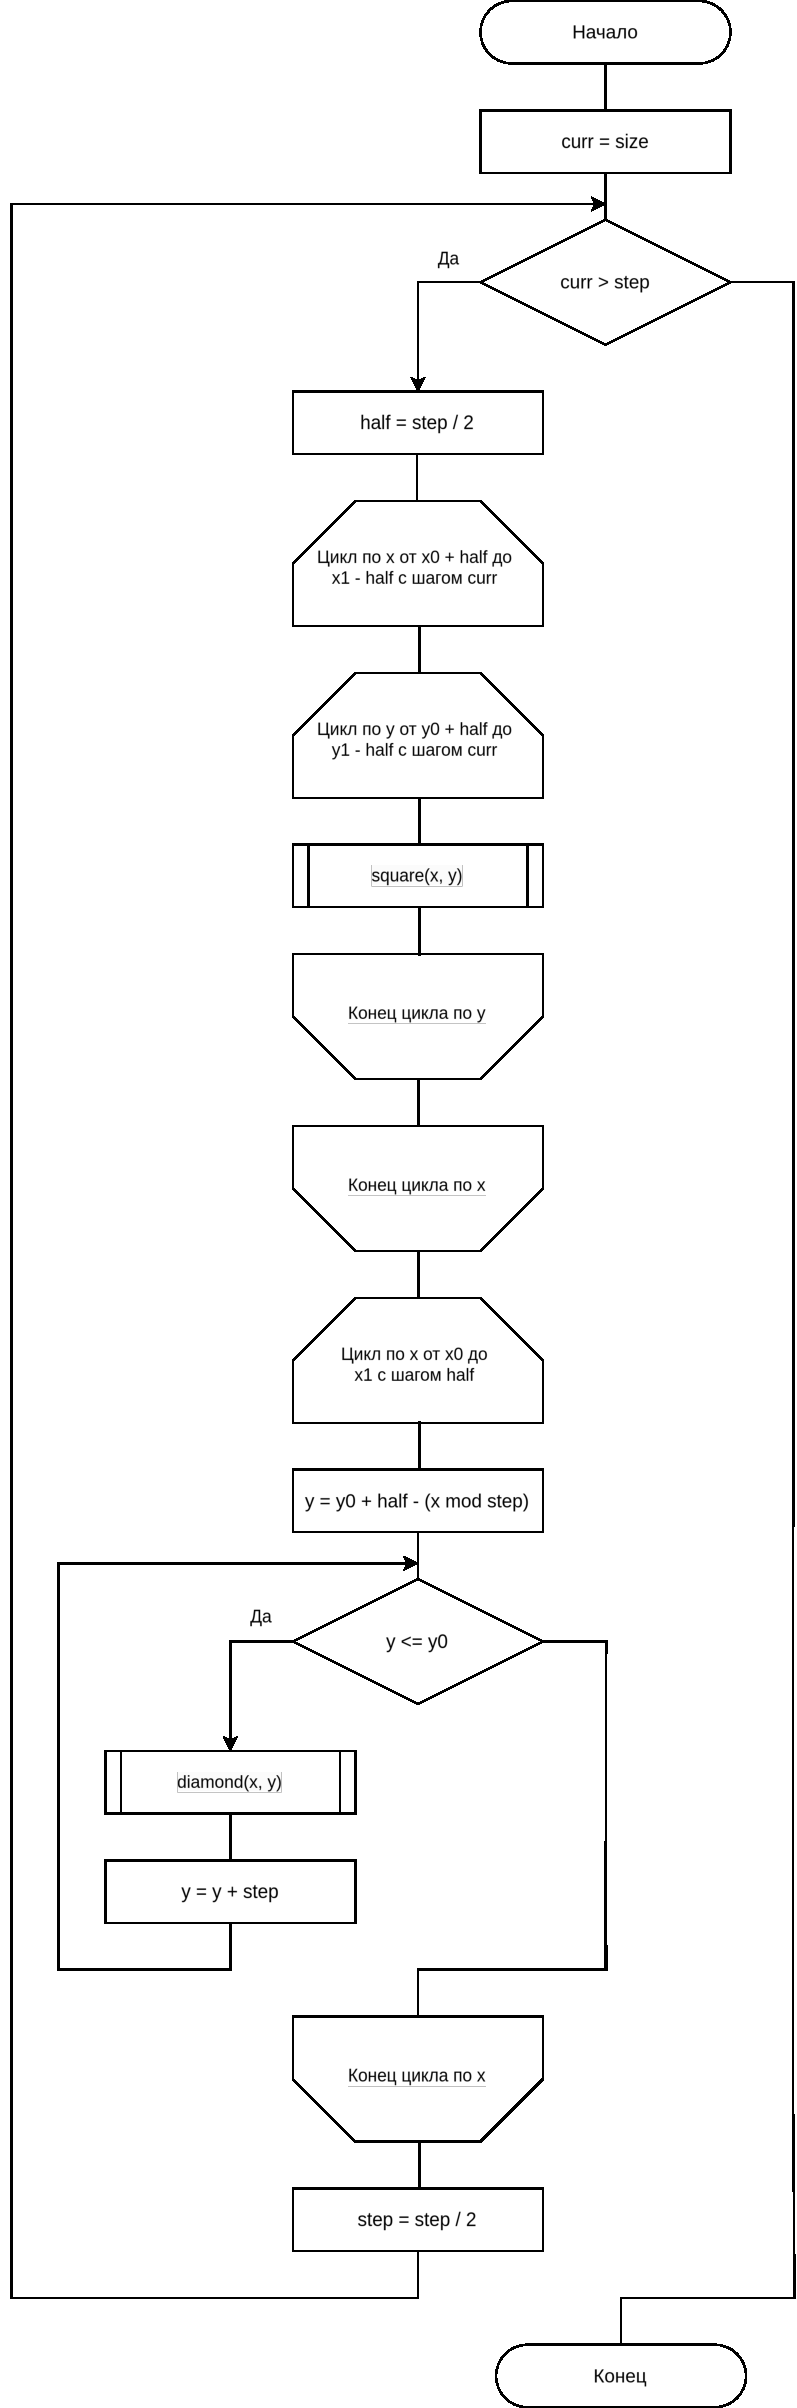
\includegraphics[width=0.3\textwidth]{tex_parts/ds-diagram.pdf}
	\caption{\label{fig:ds-scheme}Схема алгоритма diamond-square}
\end{figure}

На шаге $square$ значение в точке $(x, y)$ берется как среднее между значениями в точках $(x - 1, y - 1)$, $(x - 1, y + 1)$, $(x + 1, y - 1)$, $(x + 1, y + 1)$. На шаге $diamond$ значение в точке $(x, y)$ берется как среднее между значениями в точках $(x - 1, y)$, $(x, y - 1)$, $(x + 1, y)$, $(x, y + 1)$.  Также на каждом из шагов к полученному значению прибавляется случайное число, после чего идёт проверка на принадлежность диапазону высот.

\subsection{Шум Перлина}

В отличие от алгоритма diamond-square, в шуме Перлина отсутствует зависимость между точками, поэтому параметры нужны только для настройки генератора. Схема алгоритма поиска значения в точке представлена на рисунке \ref{fig:perlin-scheme}. 

\begin{figure}[h!]
	\centering
	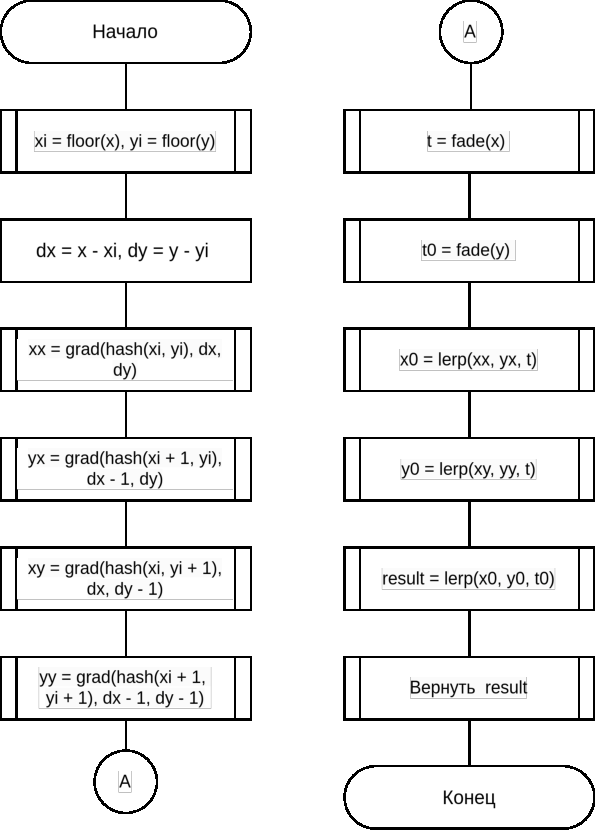
\includegraphics[width=0.5\textwidth]{tex_parts/perlin.pdf}
	\caption{\label{fig:perlin-scheme}Схема алгоритма поиска значения для шума Перлина}
\end{figure}

Здесь функция $grad$ ищет градиент вектора, $hash$ -- значение хеш-функции в точке, $lerp$ -- линейная интерполяция, а $fade$ вычисляется по формуле \ref{eq:fade}:

\begin{equation}
	\label{eq:fade}
	fade(t) = t * t * t * (t * (t * 6 - 15) + 10)
\end{equation}
 
\section{Построение кадра}

В первую очередь для каждой точки вычисляется интенсивность света $I$ по закону Ламберта (формула \ref{eq:lambert}):

\begin{equation}
	\label{eq:lambert}
	I = I_0 \cos{\phi}
\end{equation}

\noindent где $I_0$ -- интенсивность освещения от источника света, а $\phi$ -- угол между нормалью и вектором направления света.

Далее с использованием паттерна Посетитель обходятся все объекты сцены. Посетитель игнорирует источник света и камеру, а ландшафт воспринимает как паттерн Компоновщик, из-за чего обходит все квадраты, принадлежащие ландшафту. На рисунке \ref{fig:draw} изображена схема алгоритма преобразования координат перед отрисовкой для каждого квадрата. На вход подаются матрицы преобразования координат $camera\_matrix$ и $frustum\_matrix$, а также фокусное расстояние $focus$.

Матрица $camera\_matrix$ получается по формуле \ref{eq:camera}:

\begin{equation}
	\label{eq:camera}
	camera\_matrix = \begin{pmatrix}
		VX_x & VX_y & VX_z & 0     \\
		VY_x & VY_y & VY_z & 0     \\
		VZ_x & VZ_y & VZ_z & focus \\
		0    & 0    & 0    & 1     \\
	\end{pmatrix}
\end{equation}

\noindent где $VX$, $VY$ и $VZ$ -- векторы базиса камеры, $focus$ - фокусное расстояние камеры.

Матрица $frustum\_matrix$ получается по формуле \ref{eq:frustum}:

\begin{equation}
	\label{eq:frustum}
	frustum\_matrix = \begin{pmatrix}
		-f & 0      & \frac{width}{2}  & 0     \\
		0      & -f & \frac{height}{2} & 0     \\
		0      & 0      & \frac{v + f}{v} & - \frac{f(v + f)}{v}\\
		0      & 0      & 1                & 0     \\
	\end{pmatrix}
\end{equation}

\noindent где $f$ -- фокусное расстояние камеры, $v$ -- дальность прорисовки, $width$ - ширина экрана, $height$ - высота экрана.

\begin{figure}[h!]
	\centering
	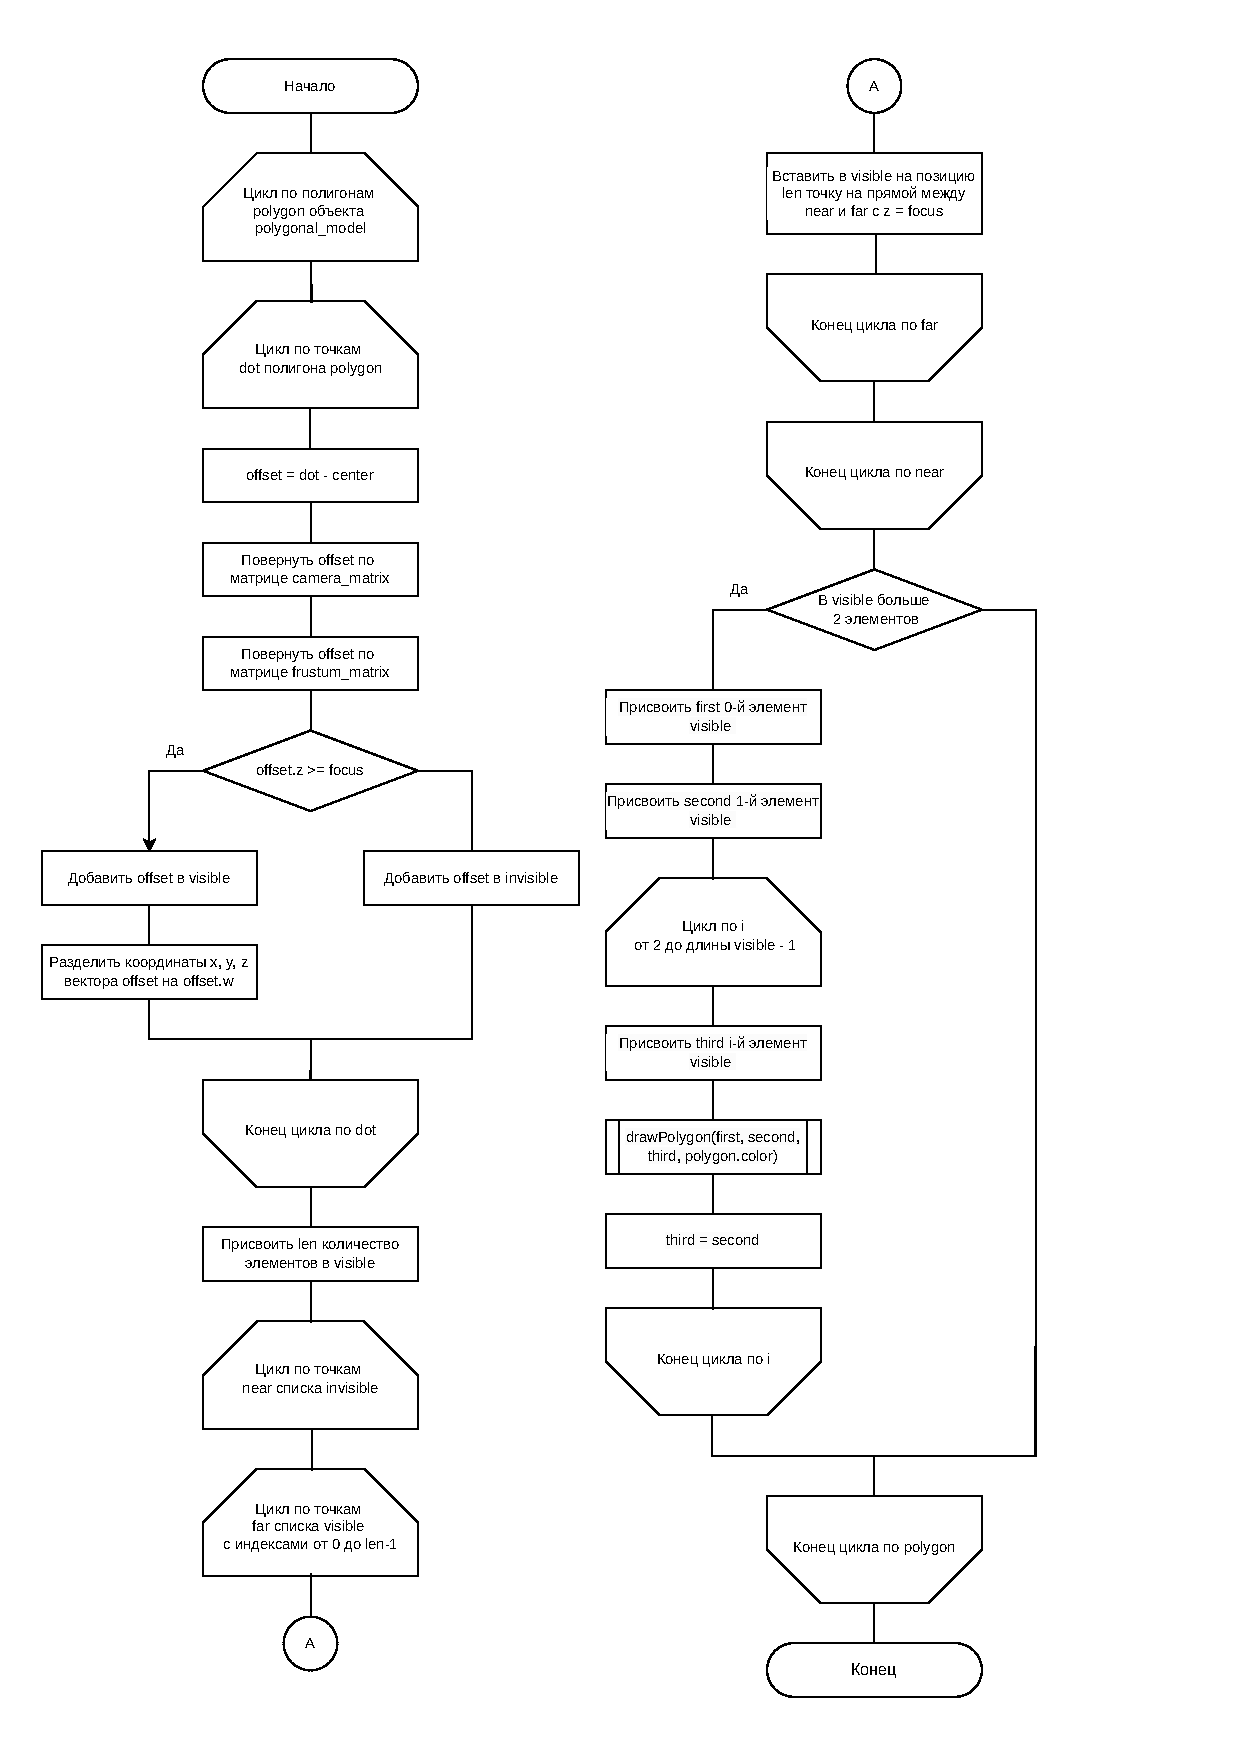
\includegraphics[width=0.6\textwidth]{tex_parts/draw.pdf}
	\caption{\label{fig:draw}Подготовка данных к отрисовке}
\end{figure}

На рисунке \ref{fig:z-buffer} изображена схема алгоритма отрисовки полигона. На вход алгоритму передаются 3 преобразованные вершины полигона $A$, $B$, и $C$, интенсивность света в них, цвет полигона $color$, Z-буфер $buffer$.

Координата $z$ произвольной точки D на плоскости ABC вычисляется по формуле \ref{eq:z}:

\begin{equation}
	\label{eq:z}
	D_z = \alpha A_z + \beta B_z + \gamma C_z
\end{equation}

\noindent где $\alpha$, $\beta$ и $\gamma$ -- барицентрические координаты точки D на плоскости ABC.

Интенсивность света $I$ в точке D вычисляется по формуле \ref{eq:I}:

\begin{equation}
	\label{eq:I}
	D_I = \alpha A_I + \beta B_I + \gamma C_I
\end{equation}

\begin{figure}[h!]
	\centering
	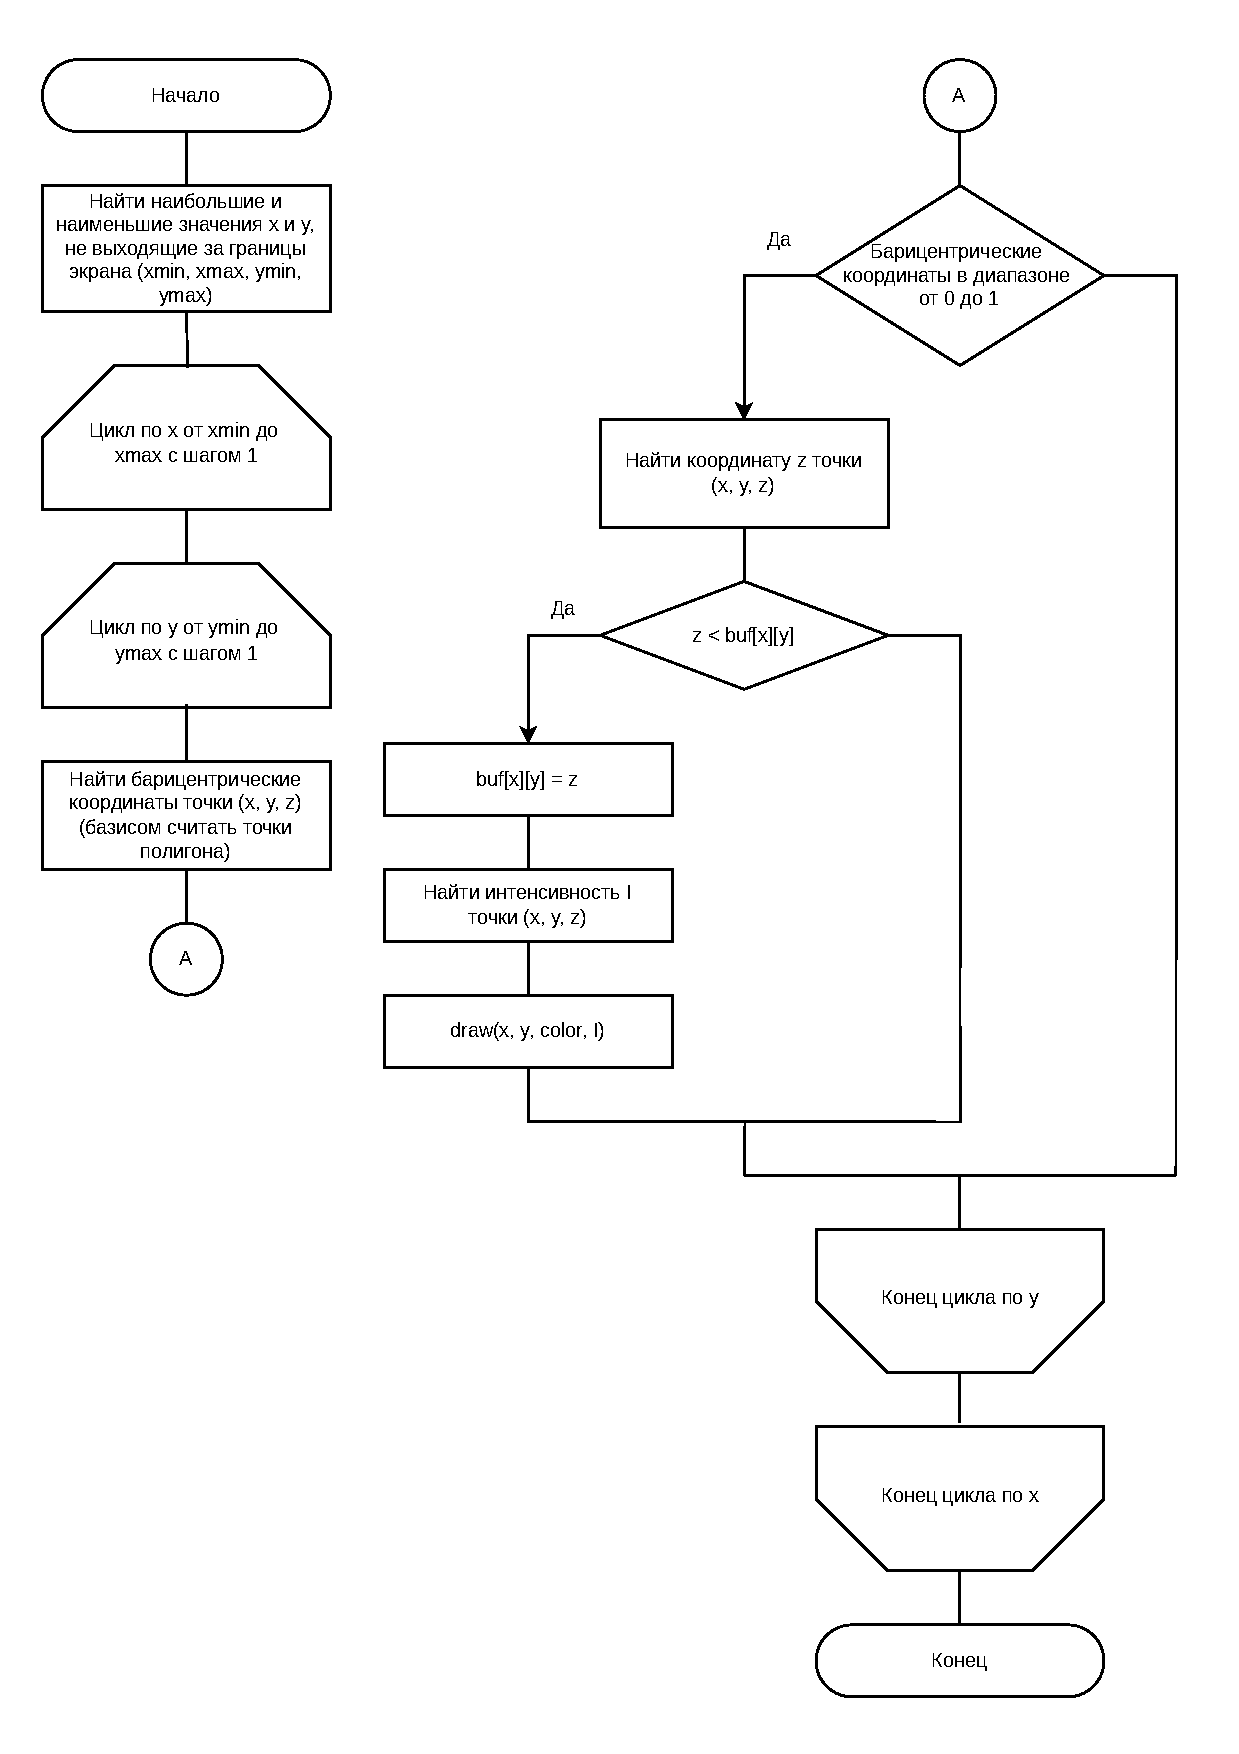
\includegraphics[width=0.6\textwidth]{tex_parts/z-buffer.pdf}
	\caption{\label{fig:z-buffer}Отрисовка треугольного полигона}
\end{figure}

\section{Выводы}

В данном разделе были выбраны структуры данных, а также построены схемы алгоритмов, функциональная схема работы программы и диаграмма классов.

